\chapter{Исследовательская часть}

\section{Технические характеристики}

Технические характеристики устройства, на котором выполнялись замеры по времени:

\begin{itemize}
    \item Процессор: Intel i5-1035G1 (8) @ 3.600 ГГц.
    \item Оперативная память: 16 ГБайт.
    \item Операционная система: Manjaro Linux x86\_64 (версия ядра Linux 5.15.131-1-MANJARO).
\end{itemize}

Во время проведения измерений времени ноутбук был подключен к сети электропитания и был нагружен только системными приложениями.

\section{Демонстрация работы программы}

На рисунке \ref{fig:prog-demo} показан пример работы разработанной программы для случая, когда пользователь выбирает опцию <<Умножение алгоритмом Винограда>> и затем~--- <<Умножение алгоритмом Штрассена>>.
Входными данными являются матрицы

\[
\begin{pmatrix}
    0 & 4 & 1 & 0 \\
    5 & 1 & 4 & 6 \\
    9 & 3 & 5 & 1 \\
    0 & 5 & 7 & 9
\end{pmatrix}
\text{и}
\begin{pmatrix}
    5 & 0 & 0 & 0 \\
    0 & 5 & 0 & 0 \\
    0 & 0 & 5 & 0 \\
    0 & 0 & 0 & 1
\end{pmatrix}
\]

\begin{figure}[H]
    \centering
    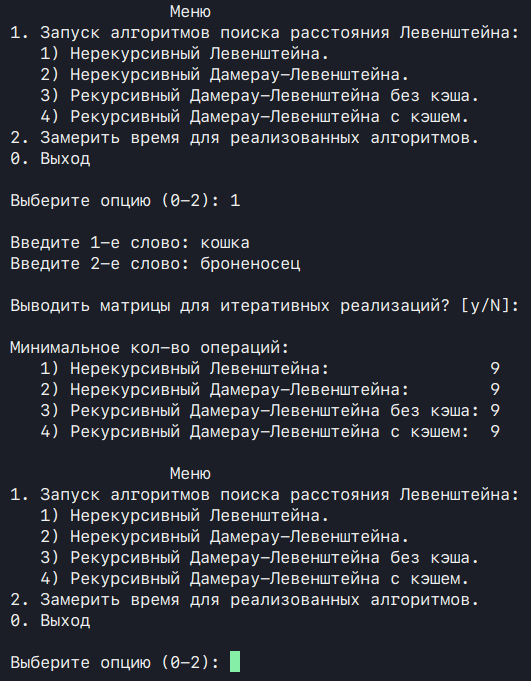
\includegraphics[height=0.6\textheight]{images/prog_demo.png}
    \caption{Демонстрация работы программы}
    \label{fig:prog-demo}
\end{figure}

\section{Временные характеристики}

Исследование временных характеристик реализуемых алгоритмов производилось три раза:

\begin{enumerate}
    \item на квадратных матрицах нечетного размера, который изменяется от 1 до 101 с шагом 10;
    \item на квадратных матрицах четного размера, который изменяется от 10 до 100 с шагом 10;
    \item на квадратных матрицах, размер которых~--- степень двойки от 2 до 128.
\end{enumerate}


В силу того, что время работы алгоритмов может колебаться в связи с различными процессами, происходящими в системе, для обеспечения более точных результатов измерения для каждого алгоритма повторялись 100 раз, а затем бралось их среднее арифметическое значение.

На рисунке \ref{fig:odd-time} показаны зависимости времени выполнения классического алгоритма умножения, алгоритма Винограда (без оптимизации и с ней) от нечетного размера квадратных матриц.

На рисунке \ref{fig:even-time} представлены зависимости времени выполнения классического алгоритма умножения, алгоритма Винограда (без оптимизации и с ней) от четного размера квадратных матриц.

На рисунке \ref{fig:strassen} представлены зависимости времени выполнения классического алгоритма умножения, алгоритмов Винограда (без оптимизации и с ней) и Штрассена от матриц, размер которых~--- степень 2.


\begin{figure}[H]
    \centering
    \includesvg[width=1.0\textwidth]{images/time/all_odd.svg}
    \caption{Результат измерений времени работы реализуемых алгоритмов на матрицах нечетных размеров}
    \label{fig:odd-time}
\end{figure}

\begin{figure}[H]
    \centering
    \includesvg[width=1.0\textwidth]{images/time/all_even.svg}
    \caption{Результат измерений времени работы реализуемых алгоритмов на матрицах четных размеров}
    \label{fig:even-time}
\end{figure}

\begin{figure}[H]
    \centering
    \includesvg[width=1.0\textwidth]{images/time/strassen.svg}
    \caption{Результат измерений времени работы реализуемых алгоритмов на матрицах, размеры которых~--- степень 2}
    \label{fig:strassen}
\end{figure}

\section{Характеристики по памяти}

Введем следующие обозначения:

\begin{itemize}
    \item $\text{size}(v)$~--- функция, вычисляющая размер входного параметра $v$ в байтах;
    \item $int$~--- целочисленный тип данных.
\end{itemize}

Теоретически оценим объем используемой памяти алгоритмов умножения для целочисленной матрицы размером $n \times n$.

\subsection{Классический алгоритм}

Оценка используемой классическим алгоритмом умножения памяти приведена в формуле (\ref{eqn:mem-classic}).

\begin{equation}
    \label{eqn:mem-classic}
    \begin{aligned}
        M_{Classic} = 3 \cdot \text{size}(int) + 3 \cdot \text{size}(int) + n \cdot n \cdot \text{size}(int) = \\
        = \text{size}(int) \cdot (6 + n^2),
    \end{aligned}    
\end{equation}
где $3 \cdot \text{size}(int)$~--- размер переменных для хранения размеров матриц,
\\ $3 \cdot \text{size}(int)$~--- размер переменных цикла,
\\ $n \cdot n \cdot \text{size}(int)$~--- размер результирующей матрицы.

\subsection{Алгоритм Винограда}

Оценка используемой алгоритмом Винограда памяти приведена в формуле (\ref{eqn:mem-classic}).

\begin{equation}
    M_{Winograd} = M_{RowFactors} + M_{ColFactors} + M_{res} + M_{mul} + M_{odd},
\end{equation}
где $M_{RowFactors}, M_{ColFactors}$~--- размер вспомогательных массивов,
\\ $M_{res}$~--- размер результирующей матрицы,
\\ $M_{mul}$~--- размер памяти, используемой при умножении матриц,
\\ $M_{odd}$~--- размер памяти, используемой при обработке условия о нечетности размеров матриц.

Размер результирующей матрицы рассчитывается по формуле (\ref{eqn:mem-result-mat})
\begin{equation}
    \label{eqn:mem-result-mat}
    M_{res} = n \cdot n \cdot \text{size}(int).
\end{equation}

Количество памяти, затрачиваемой на хранение массивов $RowFactors$ и $ColFactors$ равно
\begin{equation}
    M_{RowFactors} = M_{ColFactors} = n \cdot \text{size}(int).
\end{equation}

При умножении размер используемой памяти равен
\begin{equation}
    M_{mul} = 3 \cdot \text{size}(int),
\end{equation}
где $3 \cdot \text{size}(int)$~--- переменные цикла.


Количество памяти, затрачиваемой на обработку случая, когда матрица имеет нечетный размер, равно
\begin{equation}
    \label{eqn:mem-winograd-odd}
    M_{odd} = 
    \begin{cases}
        0, & \text{четная}\\
        2 \cdot \text{size}(int), & \text{нечетная}
    \end{cases}
\end{equation}

\subsection{Оптимизированный алгоритм Винограда}

Оценка используемой оптимизированной версией алгоритма Винограда памяти приведена в формуле (\ref{eqn:mem-classic}).

\begin{equation}
    M_{WinogradOpt} = M_{RowFactors} + M_{ColFactors} + M_{res} + M_{mul} + M_{odd} + \text{size}(int),
\end{equation}
где $M_{RowFactors}, M_{ColFactors}$~--- размер вспомогательных массивов,
\\ $M_{res}$~--- размер результирующей матрицы,
\\ $M_{mul}$~--- размер памяти, используемой при умножении матриц,
\\ $M_{odd}$~--- размер памяти, используемой при обработке условия о нечетности размеров матриц,
\\ $\text{size}(int)$~--- размер переменной, используемой для кеширования.

Размер памяти, необходимой для обработки массивов $RowFactors$ и $ColFactors$, равен
\begin{equation}
    M_{RowFactors} = M_{ColFactors} = n \cdot \text{size}(int) + \text{size}(int),
\end{equation}
где $\text{size}(int)$~--- размер переменной, используемой для кеширования.

Количество памяти, затрачиваемой на умножение, равно
\begin{equation}
    M_{mul} = 3 \cdot \text{size}(int) + \text{size}(int),
\end{equation}
где $\text{size}(int)$~--- размер переменной, используемой для кеширования.

$M_{res}$ и $M_{odd}$ рассчитываются согласно соотношениям (\ref{eqn:mem-result-mat}) и (\ref{eqn:mem-winograd-odd}) соотвественно.

\subsection{Алгоритм Штрассена}

Ниже приведена оценка количества памяти, затрачиваемой при каждом рекурсивном вызове алгоритма Штрассена.

\begin{equation}
    \begin{gathered}
        M_{StrassenCall} = (4 \cdot \frac{n}{2} \cdot \frac{n}{2} + 4 \cdot \frac{n}{2} \cdot \frac{n}{2} + 11 \cdot \frac{n}{2} \cdot \frac{n}{2} + n \cdot n) \cdot \text{size}(int) + \\
        + 2 \cdot \text{size}(int),
    \end{gathered}
\end{equation}
где $2 \cdot \text{size}(int)$~--- размер переменных, используемых для кеширования,
\\ $4 \cdot \frac{n}{2} \cdot \frac{n}{2} \cdot \text{size}(int)$~--- размер матриц, полученных в результате разбиения исходных на 4 части,
\\ $11 \cdot \frac{n}{2} \cdot \frac{n}{2} \cdot \text{size}(int)$~--- размер промежуточных матриц,
\\ $n \cdot n \cdot \text{size}(int)$~--- размер результирующей матрицы.

\section{Вывод}
\addcontentsline{toc}{section}{Вывод}

В результате исследования реализуемых алгоритмов по времени выполнения можно сделать следующие выводы:
\begin{enumerate}
    \item оптимизированный алгоритм Винограда оказался самым эффективным по времени независимо от размерности входных матриц (см. рисунки \ref{fig:odd-time} -- \ref{fig:strassen}).
    \item время работы классического алгоритма умножения и оптимизированного и неоптимизированного алгоритмов Винограда на матрицах нечетного размера больше, чем на матрицах четного размера (см. рисунки \ref{fig:odd-time}, \ref{fig:even-time});
    для алгоритма Винограда меньшая скорость работы на матрицах нечетного размера объясняется необходимостью дополнительных вычислений крайних строк и столбцов в результирующей матрице;
    \item алгоритм Штрассена показал наименьшую производительность среди всех алгоритмов, исследуемых на матрицах, размер которых равен степени двойки (см. рисунок \ref{fig:strassen});
    вероятно, низкая производительность алгоритма обуславливается необходимостью выполнения дополнительных операций сложения/вычитания, разбиения/слияния матриц;
\end{enumerate}

В результате теоретической оценки алгоритмов по памяти можно сделать вывод о том, что стандартный алгоритм умножения матриц требует наименьших расходов по памяти.
Алгоритм Штрассена, напротив, является самым требовательным по памяти за счет использования вспомогательных подматриц для выполнения рассчетов и рекурсивных вызовов.

Оптимизированный алгоритм Винограда является более ресурсозатратным, чем неоптимизированный, так как первый алгоритм использует дополнительные переменные для хранения промежуточных рассчетов.